\chapter*{General Introduction}
\addcontentsline{toc}{chapter}{General Introduction}

\section*{Context and Problem Statement}

Agriculture is one of the foundations of food security, economic development, and social stability. However, it is also one of the sectors most exposed to climate variability, water scarcity, soil degradation, and increasing production pressure. In many regions, irrigation remains a central factor determining crop quality and yield. When irrigation is applied too late, plants may suffer water stress and productivity may decrease. When irrigation is applied too early or in excessive quantities, water is wasted, soil nutrients may leach, and the cost of operation increases. The challenge is therefore not simply to irrigate, but to irrigate at the right time, with the right quantity, and according to the actual state of the soil, crop, and environment.

Traditional irrigation practices are often based on fixed schedules, manual field observation, or the farmer's experience. Precision agriculture responds to this issue by relying on sensors, communication systems, data processing, and intelligent decision support. Smart irrigation is one of the most important applications of precision agriculture because it directly addresses water-use efficiency and sustainability.

The emergence of the Internet of Things (IoT), wireless sensor networks, low-cost microcontrollers, cloud services, and artificial intelligence has transformed agricultural monitoring. Sensors can measure soil moisture, soil temperature, air temperature, relative humidity, rainfall, wind speed, wind direction, pressure, leaf wetness, and light intensity. Communication systems can transmit these measurements to a gateway or cloud platform. Machine learning models can process data and predict whether irrigation is required. Dashboards can visualize the current state of a plot and allow the farmer to control an actuator remotely. However, many smart irrigation projects remain limited to monitoring, threshold-based control, or isolated prediction models.

Digital Twin technology offers a more integrated engineering approach. A Digital Twin is not only a dashboard or a static simulation. It is a virtual representation of a physical system, continuously updated using real data, able to simulate future behavior, support decision-making, and potentially influence the physical system through feedback or actuation.

This Engineering Diploma thesis focuses on the design, implementation, deployment, and validation of Agrio, a Digital Twin-based intelligent irrigation platform for precision agriculture. The scientific background and state of the art are kept as a foundation, while the main engineering contribution is the construction of an end-to-end cyber-physical prototype.

\section*{Objectives}

The central engineering question of this thesis is: how can a Digital Twin architecture be designed and deployed to improve decision support and operational control in an intelligent irrigation system? This question is divided into secondary questions: what implementation choices are necessary to connect the physical and virtual irrigation system? How can sensor acquisition, MQTT messaging, backend processing, database persistence, machine learning inference, simulation, user interfaces, scheduling, and pump control be integrated in one coherent platform? How can the prototype be validated technically in a controlled experimental environment?

The objectives of the Engineering Diploma thesis are: to design a complete architecture for an intelligent irrigation Digital Twin; to implement IoT data ingestion using MQTT; to store agricultural measurements and system states in a structured database; to integrate machine learning for irrigation prediction; to simulate moisture evolution under alternative scenarios; to generate irrigation recommendations; to support human validation and scheduling; to control a physical water pump through a WeMos device; and to deploy and validate the platform as a working prototype.

The main contribution is technical. The project implements an end-to-end prototype connecting Libelium sensors, XBee RF, Raspberry Pi, MQTT, FastAPI, PostgreSQL, Random Forest inference, Digital Twin simulation, web/mobile interfaces, and pump control. The project therefore demonstrates a practical path from research concepts to an operational cyber-physical prototype.

\section*{Thesis Outline}

The thesis is organized according to the Engineering Diploma structure. The front matter contains the acknowledgements, abstracts, and lists. The introduction presents the context, problem statement, objectives, and outline. The background and state-of-the-art chapters introduce precision agriculture, smart irrigation, Digital Twins, IoT, artificial intelligence, related works, and scientific positioning. The contribution part presents requirements, conception, design, architecture, implementation, Digital Twin and AI pipeline, user interfaces, deployment, validation, and discussion. The thesis ends with a general conclusion and future perspectives.

\begin{figure}[H]
    \centering
    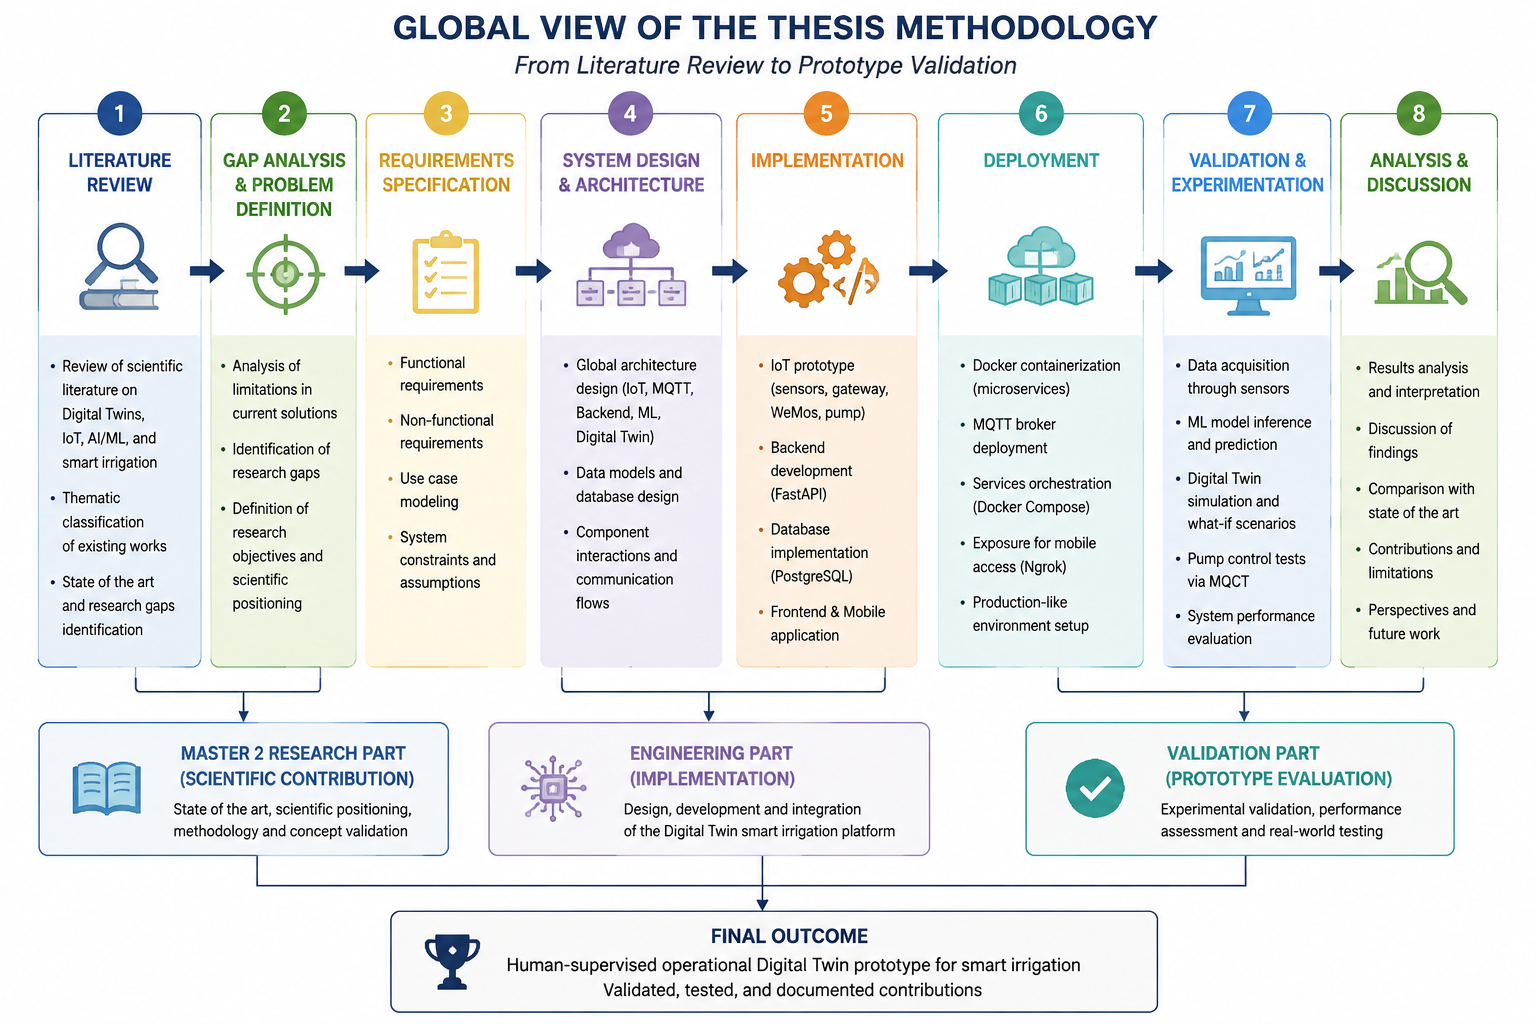
\includegraphics[width=0.9\textwidth]{figures/cover/Figure 0.1 — Global view of the thesis methodology from literature review to prototype validation.png}
    \caption{Global view of the thesis methodology from literature review to prototype validation. Source: Authors.}
    \label{fig:0-1-global-view-of-the-thesis-methodology-from-literature-review-to-pr}
\end{figure}

\begin{footnotesize}
\setlength{\tabcolsep}{2pt}
\begin{longtable}{@{}>{\raggedright\arraybackslash}p{0.28\textwidth}>{\raggedright\arraybackslash}p{0.28\textwidth}>{\raggedright\arraybackslash}p{0.28\textwidth}@{}}
\caption{Summary of Engineering Diploma objectives and contributions}\\
\toprule
Dimension & Objective & Contribution \\
\midrule
\endfirsthead
\toprule
Dimension & Objective & Contribution \\
\midrule
\endhead
Architecture & Design an end-to-end Digital Twin irrigation architecture & Layered system connecting sensing, MQTT, backend, database, ML, simulation, dashboard, and pump \\
Implementation & Build the Agrio prototype & FastAPI, PostgreSQL, HiveMQ/MQTT, Random Forest service, Next.js dashboard, Flutter app, WeMos control \\
Deployment & Run the platform as an integrated system & Docker Compose deployment and service organization \\
Validation & Demonstrate the technical workflow & Evidence through MQTT payloads, database readings, dashboard updates, simulation outputs, and actuator status \\
\bottomrule
\end{longtable}
\end{footnotesize}
